\section{PDF Parsing}
\label{sec:parsing}

%%%%% Trust Chain subsection %%%%

\subsection{Data Dependencies in PDF Parsing (the Trust Chain)}
\label{sec:trust-chain}

\begin{figure}[t]
  \centering
  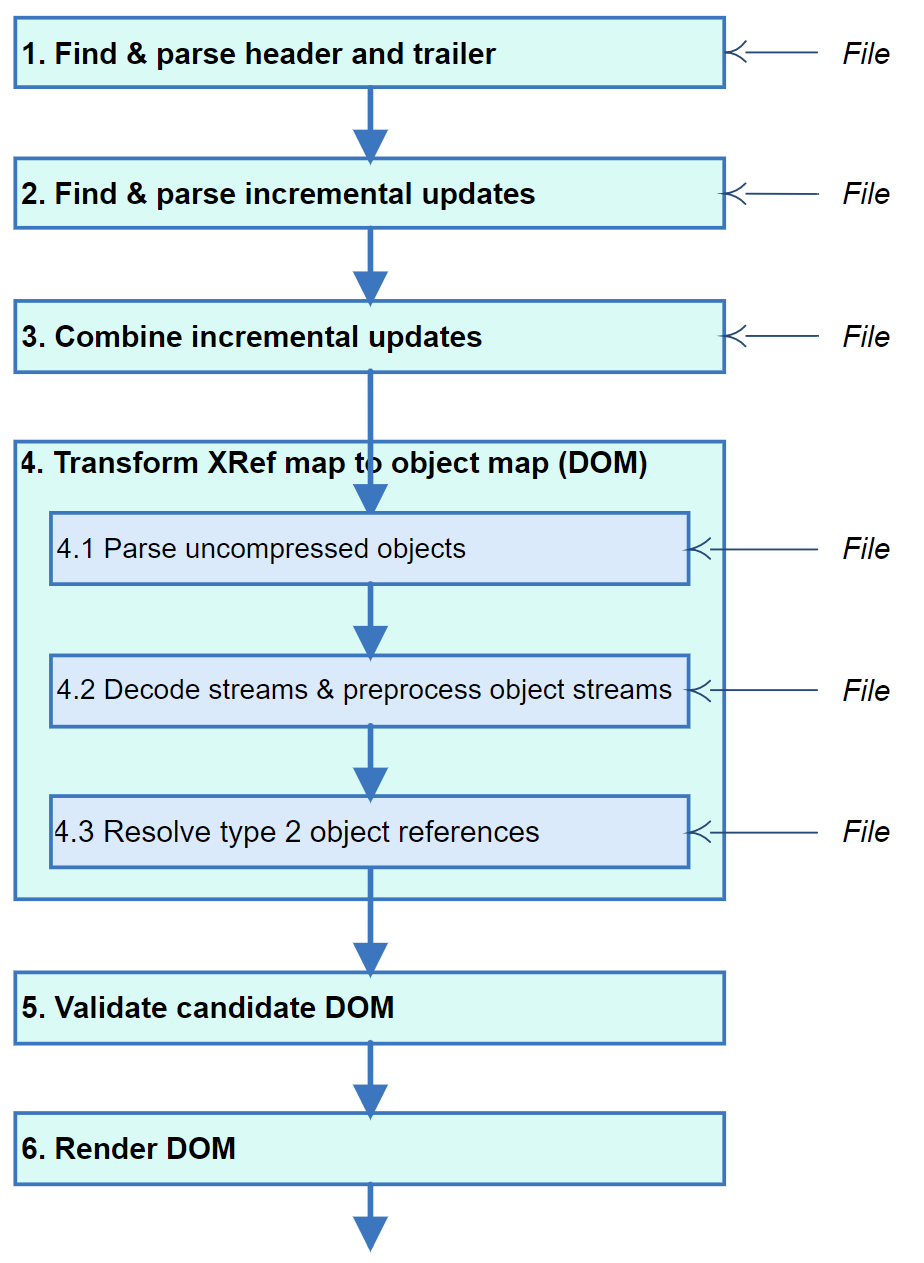
\includegraphics[width=0.8\linewidth]{figures/Stages.png}
  \caption{Stages of PDF Parsing (i.e., the Trust Chain).}
  \label{fig:pdf-trust-chain}
\end{figure}

We have touched upon the complexities of parsing PDF, but to
appreciate these, one has to understand the dependencies and
interactions between the features.  The main stages
(\cref{fig:pdf-trust-chain}) include:
%
\begin{itemize}
\item \textbf{Stage 1}: Find and parse both the PDF header and the PDF trailer to locate
  the document trailer dictionary and the start of the \emph{last} incremental update, or
  the cross reference table of the original document in the case of no updates.
\item \textbf{Stage 2}: Find and parse each cross reference table or incremental update. 
  Note that this stage uses context from Stage 1 (such as the file offset and trailer
  information) in order to know \emph{where} and \emph{how} to parse.
\item \textbf{Stage 3}: Compute the XRef map of the final PDF, by
  accounting for each set of edits performed by an incremental
  update.
  %
  Depending on the laziness of stage 2, this stage may need to further
  parse the input file.
 \item \textbf{Stage 4}: Transform the XRef map to an object map.
   %
   This stage is complex, requiring three sub-stages that each parse
   the input file (see \cref{sec:specifying}).
   %
   Upon success, this stage yields a candidate DOM with valid syntax.
 \item \textbf{Stage 5}: Validate that the candidate DOM represents a
   document graph with valid \emph{semantics}.
   % 
   Only the partially validated DOM, as a mapping from object
   references to syntactically valid PDF objects, can be the subject
   of validating of semantic properties such as dictionaries binding
   expected keys to values of expected types and freedom from
   unresolvable references.
   \begin{comment}
     BH: recommend cutting: seem more confusing than it's worth:

     text stream objects are syntactically valid, no unexpected
     recursion,
   \end{comment}
\item \textbf{Stage 6}: Render the validated DOM, or selected
  segments, in the required final representation.
\end{itemize}

Any error (malicious or otherwise) in earlier stages can affect the
output of stages that follow.
%
Note that stages 2, 3, 4.1, 4.2, and 4.3 all depend on inputs from
previous stages to determine where and how to parse segments of the
PDF input file.
%
Errors that percolate into these stages can cause all forms of havoc
(parsing wrong or out-dated data, etc.).

% compare to single-stage design:
An implementation could potentially merge stages 2, 3, 4.1, 4.2, 4.3,
providing a superficial simplicity.
%
However, our eventual argument (see \cref{sec:single-pass-problems})
is that such an implementation would be overly complex and result in a
design for which it is difficult to determine if it correctly
implements the standard and to determine that it terminates for all
input files.

%
Although \emph{Validate candidate DOM} (stage 5) is expansive, the
properties that it must validate are well defined by the 
PDF standard.
%
Validation in this stage involves ensuring that each individual PDF
object binds all the required keys to appropriate values in the context
of its reference in the DOM.
%
E.g., a \emph{thumbnail} object must be an Image XObject and bind the
required keys \lstcd{Height} and \lstcd{Width} to non-negative
integers.
%
A reference expected to refer to a thumbnail that refers instead to a
non-thumbnail object (e.g., a font dictionary) is valid in only
syntactic---but not semantic---terms.
%
Recent work~\cite{peterwyattArlingtonPDFModel2021} has resulted in the
first specification-derived comprehensive machine-readable model of
every object, their attributes and relationships in the PDF DOM. The
use of such a model for code generation, DOM validation, or test case
generation can significantly reduce the tediousness.
%
\emph{Render DOM} (stage 6) contains its own complexities, including
rendering a PDF page as pixels for display or extracting text,
depending on context.

This paper does not further discuss stages 5 and 6, focusing instead
on stages 1 to 4, referred to as \emph{pre-DOM} parsing or
computation.  We chose to focus on Stages 1 to 4 as they have been given
little emphasis and are the source of multiple vulnerabilities.
%
Errors in these stages can compromise the correctness of the complete
format definition, even if later stages are defined as intended when
viewed in isolation.

%%%%%%%%%%%%%

We have been using ``PDF Trust Chain'' to refer to the sequence of dependent
parsers in \cref{fig:pdf-trust-chain}, although
the term \emph{Trust Chain} (or ``Chain of Trust'') is
overloaded with similar meanings in different contexts:
e.g.,
\emph{digital certificates}: a sequence of certificates signing certificates,
starting with a root certificate;
\emph{supply chain}: a product is no more reliable or secure than its
outsourced components;
\emph{trusted boot}: unless the boot-loader is correct and non-malicious,
there can be no possibility of the operating system being the same;
\emph{software stacks}: upper layers are dependent upon lower layers (such as
system libraries) and vulnerabilities at the lower layers affect all higher
layers.
The common idea is that we have layers (or components) that rely
on lower layers (sub-components) for their validity.  In other words,
{\textbf{a flaw in one layer of the trust chain causes every higher
    layer to be untrustworthy!}}

%%%%%%%%%%%%%

The intentions behind the term \emph{Trust Chain} are
%
\textbf{(1)} to highlight the many dependent stages in PDF processing;
%
\textbf{(2)} to highlight the importance of ensuring the pre-DOM
parsing, data integrity relationships and computation (the base of our
Trust Chain) is correct and secure;
%
\textbf{(3)} to remind that the integrity of the DOM cannot be
verified independently of verifying all earlier stages; and
%
\textbf{(4)} to illustrate that while PDF holds various unique
features, it follows a general pattern that may be used to understand
formats broadly.


%%%%%%%%%%%%%%%%%%%%%%%%%%%%%%%%%%%
\subsection{Parsing PDF: The details}
\label{sec:parsingfile}

We described the physical structure of a PDF file in \Cref{sec:pdf},
but the processing sequence may not be apparent.
The following paragraphs describe the processing necessary to correctly parse a PDF file containing incremental updates.

PDF parsing begins by locating the PDF Header, as it is not uncommon for PDF files to have 
preamble bytes (such as an HTTP header, HTML or XML). The offset to the start of the PDF file 
(PDF offset zero)
within a physical file can then be determined from the \lstcd{\%} sign in \lstcd{\%PDF-x.y}. 

Processing continues by seeking to the end-of-file and 
locating the \emph{last} \lstcd{startxref} keyword,
a numeric value is then parsed (giving us a byte offset 
to the last cross-reference table in the PDF).
It should be verified that \lstcd{\%\%EOF} follows the numeric value.
%
Note that this requires parsing \emph{backwards}
which is unnatural for data definition languages as well as many programming
languages;
this is a proven source of parser differentials. 
The offset to the cross-reference table must be adjusted 
for any preamble bytes prior to the PDF Header.

The parsing sub-language depends on the form of the incremental update, with
conventional cross-reference tables being simpler and largely independent of
other processing. Cross-reference streams however are more complex as they are
often compressed and thus require the pre-DOM parser to ``trust'' the stream
extent dictionary data.

The parser must then locate either the \lstcd{xref} keyword for
conventional PDF cross-reference tables, or a cross-reference stream, identified by tokens of the form \lstcd{x y obj} . 
A parser must then determine if the PDF object is a
semantically valid cross-reference stream by further parsing the stream extent dictionary and 
validating the necessary key/value pairs and also recognizing the \lstcd{stream} keyword after the dictionary end token \lstcd{>>} and the \lstcd{endstream} keyword (see \cref{fig:XRefStm}). 

In the case of conventional PDF
cross-reference tables, after the cross reference table will be the
trailer dictionary, identified by the \lstcd{trailer} keyword. 
Note that this algorithm is at
odds with the file structure as defined in the PDF standard: the Trailer section is formally defined
to contain the trailer dictionary and \lstcd{startxref} keyword, yet the parsing algorithm
requires locating the first trailer \emph{after} the end of the cross-reference table 
(versus the last trailer dictionary above the \lstcd{startxref} keyword). 
Alternatively for PDF 1.5 and later files with cross-reference
streams, the trailer dictionary data will be in the stream extent
dictionary of the cross reference stream. 

Any previous cross-reference data is identified by the value of the \lstcd{/Prev} entry in either
the trailer dictionary or the stream extent dictionary of a cross-reference stream. The
value of the \lstcd{/Prev} key is the byte offset to the immediately
preceding cross-reference data which, again, can either be a conventional
cross-reference table and to the start of the \lstcd{xref} keyword, or to a
cross-reference stream. This process repeats, working from the most recent incremental
update back through time to the original PDF document.

In each incremental update, the trailer dictionary is required to duplicate all keys from the previous
trailer and update accordingly. Of particular note is the \lstcd{/Size} entry, which must be
one greater than the largest object number allocated in the PDF file. Objects with numbers greater
than \lstcd{/Size} are defined to be the special PDF \lstcd{null} object.

Data in each cross reference table must be parsed to
identify the byte offset to the start of each PDF object, whether this be a file offset to an 
indirect object in a Body section, or a relative object position within an object stream (and 
where the object position is transformed to a byte offset within the object stream from the 
first line of text in the object stream). Note also that with conventional PDF cross-reference 
tables there is no definition for the byte offset to the end of an object, however for cross-reference 
streams this can be pre-determined.

%%%%%%%%%%%%%%%%%%%%%%%%%%%

\subsection{Specifying a Parser, not Specifying a Validator}
\label{sec:spec-approach}

\begin{figure}[t]
    \centering
    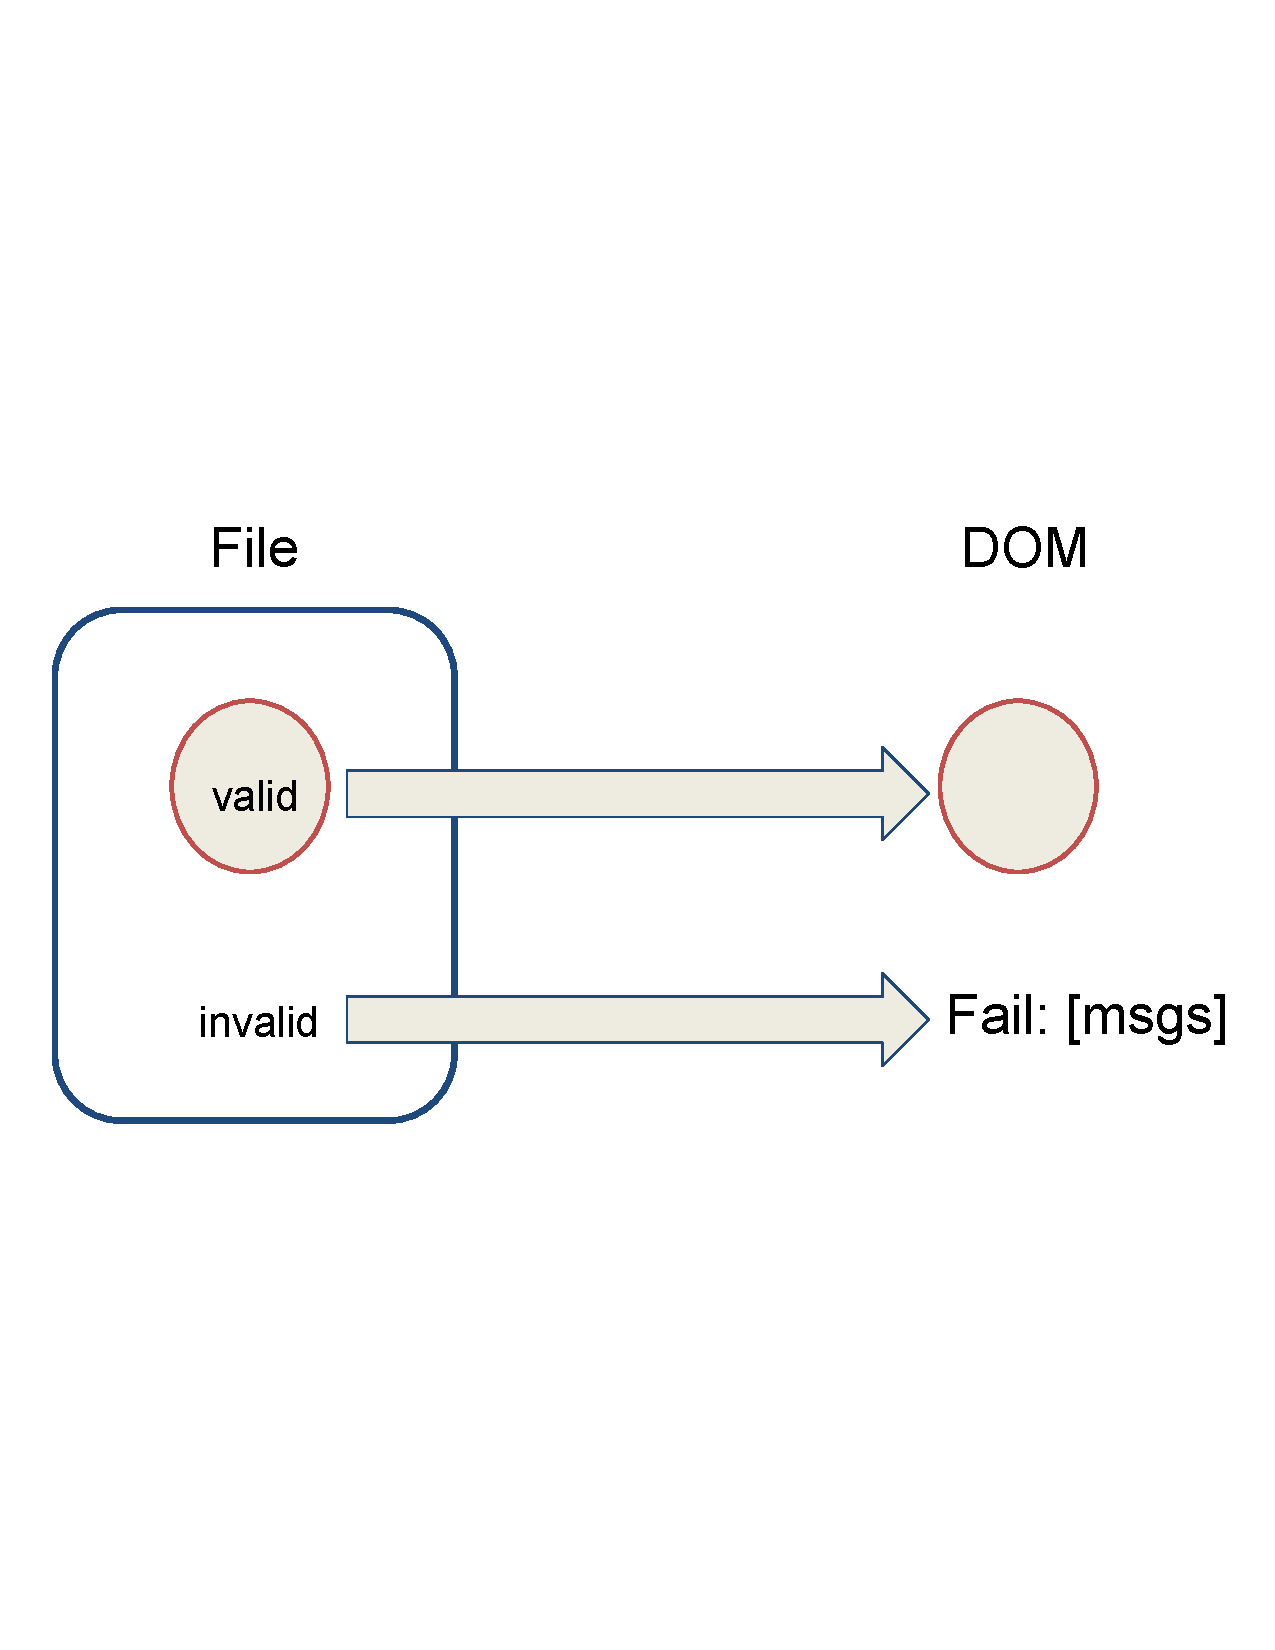
\includegraphics[width=0.50\linewidth]{figures/validator.pdf}
    \caption{Validator}
    \label{fig:validator}
    
    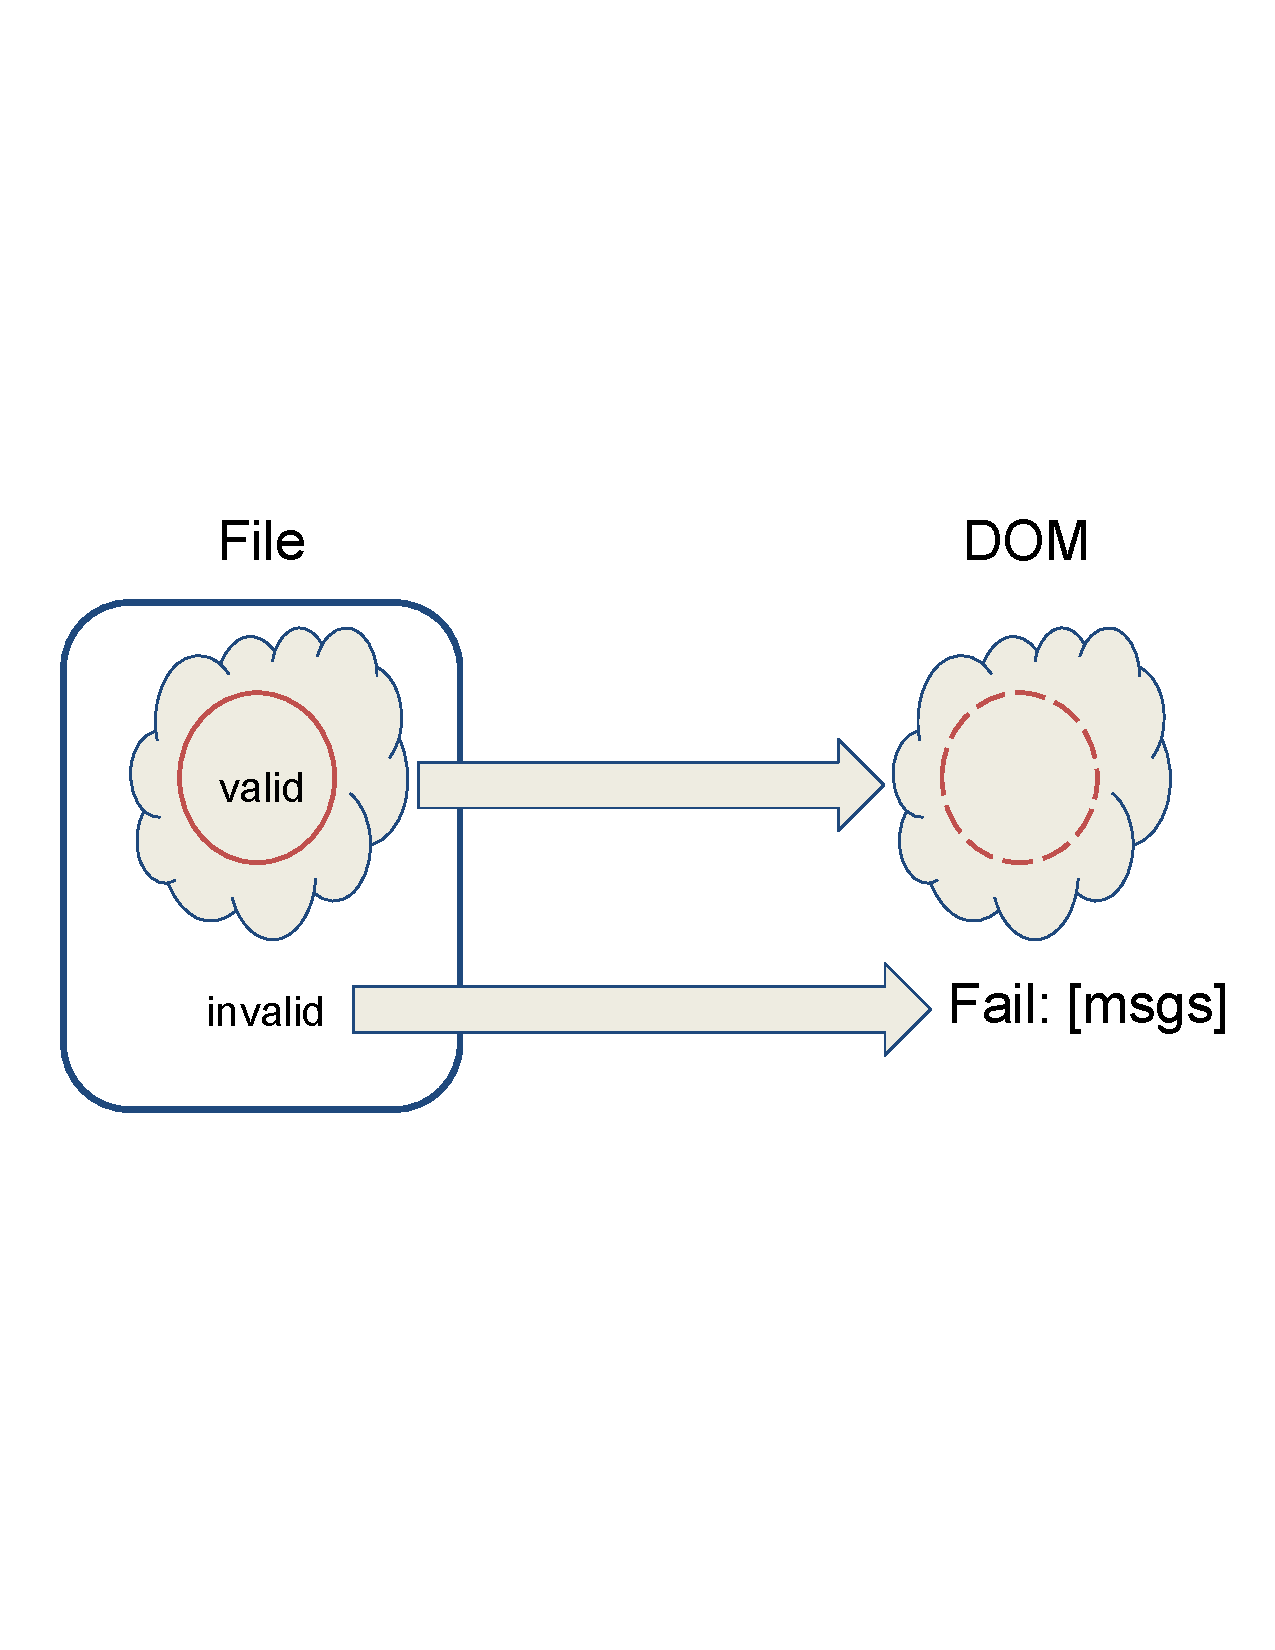
\includegraphics[width=0.50\linewidth]{figures/parser.pdf}
    \caption{Parser}
    \label{fig:parser}
\end{figure}

A \emph{key} idea in the DARPA-funded ``SafeDocs'' program is to
understand and
capture extant---used in the wild---PDF parsers.  Creating an implementation
that perfectly matches the PDF specification is not particularly useful
and would only parse a small fraction of extant PDF files.

See \Cref{fig:validator} where we show a validator (or a format \emph{recognizer}),
its function is to produce a DOM when we have a valid PDF, it must fail
otherwise.  Compare this to figure \Cref{fig:parser} where we show a parser
which has a {\bf{completely different requirement}}: to efficiently construct
the correct DOM when given an valid PDF.  A \emph{parser} is willing, if not
happy, to accept files beyond the pale of PDF.
In the \emph{parser} diagram,
we use a cloud to suggest that for various parser tools,
each is going to accept a different subset due to
\begin{itemize}
\item redundancies in the format allow for different choices,
\item the tools do not interpret the Standard uniformly,
\item tools may traverse and evaluate implicit data structures differently, and
\item tools differ in how they allow for ``minor'' errors or do error recovery.
\end{itemize}
Our goal for a \emph{parser specification} is to encompass any reasonable and
correct ``cloud''.  This goal is somewhat subjective, but generally this will
imply that we attempt to capture the laziness of various tools that only parse
or validate values upon demand.

% 
% A useful format specification must resolve a fundamental conflict between pr% ecision and restrictiveness.
% %
% An overly permissive specification, specifically of the PDF pre-DOM,  would % permit multiple compliant processors to produce radically different results,%  and thus would provide little ultimate assurance to format users.
% %
% Conversely, a specification that formalized all aspects of the standard rela% ted to pre-DOM components would prohibit almost all practical document proce% ssors, which almost never need to fully validate a document.

However, at the same time, it would be very desirable to
write a single piece of code from which we could extract
both a \emph{parser} as well as a \emph{validator}.
% our solution:
To resolve this conflict, we have %
\textbf{(1)} specified an implementation to be \emph{lazy} whenever possible;
in other words, whenever possible it defers the reading, parsing, and validation
of data; and %
\textbf{(2)} extended this specification
with separate \lstcd{validate} predicates that, when executed,
would extend our implementation to form a complete validator.

%
% Because no implementations validate documents fully, and some implementations
% are surprisingly lazy, we want our specification to be very lazy.
% %
% Due to various redundancies in PDF, there is no one exact
% laziest semantics, but we attempt to create something reasonable.
% %
% The lazier we make our spec (while remaining correct),

One of our objectives is to test implementations
with respect to our parser specification;
we would test by validating that when an implementation produces a DOM,
that DOM is equivalent to the DOM produced by the specification.
This is why we want our specification to be lazier than most implementations.

% % introduce formal specification:
% We say that a specification is \emph{formal} if it is expressed in a languag
% e whose semantics is amenable to a mechanizable definition.
% %
% By their nature, such definitions can offer precision of meaning that is a
% significant departure from standards expressed purely in prose;
% %
% in particular, they can provide a basic assurance that they do not rely on 
% undefined terms.
% %
% While their existence does not immediately solve all of the above issues in 
% format design, they are valuable artifacts for clarifying
% standards, understanding vulnerabilities, and aiding implementors.
